% ---------------------------------------------------------------------
% Das Dokument kompiliert mit pdflatex und ist auf Basis 
% von Koma-Script entstanden. 
%
% Autor des Templates (für Anmerkungen): 
% Michael von Riegen, riegen@informatik.uni-hamburg.de
%
% Einzelne Code-Teile für das Titelblatt sind aus dem Template 
% von Benjamin Kirchheim entnommen.
%
% 25.05.09, Frank Langanke: Vorlage auf aktuelle KOMA-Version aktualisiert
% 26.05.09, Michael von Riegen: Anmerkung --> aktuelles Koma-Script ist nötig!
% 17.10.2016 neues Uni logo
% ---------------------------------------------------------------------
\documentclass[11pt,DIV=15,BCOR=20mm,bibliography=totoc]{scrbook}

% Import von Paketen und Optionen die das gesamte Dokument betreffen
% sind in myPreamble.sty ausgelagert.
\usepackage{myPreamble}
\usepackage{graphicx}
\usepackage{float}
\usepackage{listings}
\usepackage[sorting=debug]{biblatex}
\addbibresource{Bachelorarbeit.bib}
\usepackage{wrapfig}
\usepackage{subfig}
\usepackage{siunitx}
\usepackage{tabularx}
\graphicspath{ {./images/} }
\usepackage{xspace}

\newcommand{\fremdwort}[1]{\emph{#1}}
\newcommand{\iic}{I\textsuperscript{2}C\xspace}
% Arbeitet man nur an einem Kapitel, wird durch folgenden Befehl nur dieses eingebunden.
% Spart manuelles auskommentieren von vielen include-Befehlen;
% hat keine Auswirkung auf input-Befehle
% \includeonly{kapitel1}
\DeclareTOCStyleEntry[%
  level=\chaptertocdepth,%
  beforeskip=0pt plus .2pt,%
  indent=0pt,%
  numwidth=1.5em,%
  entryformat=\textbf,%
  pagenumberformat=\textbf,%
  linefill=\hfill
]{tocline}{fmchapter}
   
\begin{document}

% TITELSEITE
\begin{titlepage}

	% Fehler "destination with the same identifier" unterdrücken...
  \setcounter{page}{-1}

	% Titelseite
	\begin{figure}[h]
		\begin{minipage}[b]{62mm}
			\includegraphics[width=62mm]{images/unilogo}
		\end{minipage}
		\hspace{4cm}
		%\begin{minipage}[b]{59mm}
		%	\includegraphics[width=59mm]{images/minlogo}
		%\end{minipage}
	\end{figure}

	\vfill
	
	\begin{center}
		% Diplomarbeit 
		\noindent { \huge
			Bachelorarbeit \\
		}
		\vspace{14mm}
		% Titel
		\noindent \textbf{\huge
		  Entwicklung eines Prototypen für einen 
		}
		\noindent \textbf{\huge
		  Datenhandschuh basiert auf IMUs 
		}
		\\
		\noindent \textbf{\huge
		  - Version 2
		}
		\vspace{60mm}	
	\end{center}
	
	\vfill
	
	\noindent \textbf{Can Bagdas} \\
	\noindent \rule{\textwidth}{0.4mm} 
	\noindent{\textrm{can.bagdas@studium.uni-hamburg.de}} \\
	\noindent{\textrm{Studiengang Informatik}} \\
	\noindent{\textrm{Matr.-Nr. 6726929}} \\
	\begin{tabbing}
	\hspace{8em} \=  \kill
	Erstgutachter: \> Dr. Norman Hendrich \\
	Zweitgutachter: \> Philipp Ruppel \\
	~ \\
	Abgabe: 19.04.2022
	\end{tabbing}
	
	% Rückseite der Titelseite mit Zitat
	\newpage 
	\thispagestyle{empty}
	\setcounter{page}{0}

	% wenn man Lust auf ein Zitat hat...
	% ... ansonsten auskommentieren
	~\\ \vfill \noindent 
\end{titlepage}



% VERZEICHNISSE (Inhaltsverzeichnis, Abkürzungen)
% Vorspann einleiten --> Seitennummerierung römisch
\frontmatter

% Inhaltsverzeichnis
\tableofcontents
\cleardoublepage
\chapter*{Abkürzungen}\addcontentsline{toc}{fmchapter}{Abkürzungen}
\vspace{-1cm}
{
\begin{tabularx}{\textwidth}{@{}>{\bfseries}rX@{}}
    \toprule
    3D & 3-dimensional \\
    AR & \fremdwort{augmented reality}, erweiterte Realität \\
    DoF & \fremdwort{degrees of freedom}, Freiheitsgrade\\
    MEMS & \fremdwort{microelectromechanical system}\\
    GND & \fremdwort{ground}, Masse, Bezugspotenzial \\
    \iic & \fremdwort{Inter-Integrated Circuit} (serieller Datenbus)\\
    SPI & \fremdwort{Serial Peripheral Interface} (serieller Datenbus)\\
    IMU & \fremdwort{inertial measurement unit}, inertiale Messeinheit\\
    ROS & \fremdwort{Robot Operating System}\\
    SCL & \fremdwort{signal clock}, Taktleitung bei \iic \\
    SDA & \fremdwort{signal data}, Datenleitung bei \iic \\
    UDP & \fremdwort{User Datagram Protocol} (Transportprotokoll) \\
    VCC & \fremdwort{voltage at the common collector} (Versorgungsspannung) \\
    VR & \fremdwort{virtual reality}, virtuelle Realität\\
    \bottomrule
\end{tabularx}
}
% Hauptteil einleiten --> Seitennummerierung wieder arabisch
\mainmatter

% -----------------------------------------------------------------------
% -----------------------------------------------------------------------
% -----------------------------------------------------------------------
% Einleitung
% -----------------------------------------------------------------------
% -----------------------------------------------------------------------
% -----------------------------------------------------------------------
\chapter{Einleitung}

Das Thema dieser Abschlussarbeit wird die Modellierung und den Bau zweier Datenhandschuhe umfassen. Zunächste wird eine Einleitung zu diesem  Thema beschrieben, mit einer Zielsetzung und dem Ablauf des Projektes. Welchen Anwendungsbereich und was für  Abgrenzungen stattfinden werden

\section{Zielsetzung}
Diese Arbeit wird sich damit beschäftigen, zwei Datenhandschuh aus drei unterschiedlichen Sensormodellen zu entwickeln basierend aus den Daten von integrierten IMUs an den Fingern und dem Handrücken. Dieses hängt direkt an der Abschlussarbeit von Paul Bienkowski und Carolin Konietzny an und wird eine zweite Version des ähnlichen Handschuhes mit Verwendung von drei verschiedenen IMU Typen. Das Ziel dieser Bachelorarbeit wird es sein, zwei funktionierenden Datenhandschuhe zu entwerfen, die für das Aufzeichnen von menschlichen Handbewegungen dienen und für den eventuellen Gebrauch als Fernsteuerung für eine Roboterhand. Im zweitens Teil werden beide IMU Typen für die Finger verglichen und ausgewertet.

Zusammenfassend werden diese Punkt bearbeitet:
\begin{itemize}
\item Entwicklung von zwei Datenhandschuhe basierend aus IMU Sensoren mit den Modellen MPU-6050 und BMI160 für die Finger Sensoren und dem MPU-9250 für den Handrücken.

\item Vergleich des MPU-6050 und BMI160 auf Anwendung der Genauigkeit und Fehlertoleranz. 

\item Verwendung des Sensormodelles MPU-9250, mit Benutzung des Magnetometers neben Gyroskope und Accelormeter.

\end{itemize}

Diesbezüglich werde ich auch genauer auf die einzelnen Module und Komponenten des Datenhandschuhes eingehen. Wie die Sensormodelle funktionieren, welche Vorteile der Datenhandschuh gegenüber den anderen schon existierenden Datenhandschuhe hat und was für eine Software-Architektur ich hierfür verwendet habe.

\section{Anwendungsbereich}
Das Projekt soll für zukünftige Anwendungen am Informatikum zur Verfügung stehen, im Bereich Robotik und weiteren ähnlichen Gebieten mit der Möglichkeit diesen zu erweitern. 

\section{Abgrenzung} 

Der Umfangreiche aspekt dieser Arbeit kann weit ausgebaut werden, jedoch wird diese Arbeit sich nur auf bestimmte Bereiche auseinander setzen. Hierbei wird es sich nur um einen Prototypen handeln und um keinen vollständigen Produkt. 
Dabei werden folgenden Abgrenzungen eingehalten:

\begin{itemize}
\item Es wird stark auf Modularität gesetzt, wobei ein stabiler und einzelner Handschuh nicht gebaut wird. Für den Gebrauch an unterschiedlichen Handtypen werden mehrere Komponenten gebaut, um diese anpassbar zu gestalten, wobei der Handschuh deswegen komplexer gebaut ist.

\item Visuelles tracking mit dem Handschuh wird nicht berücksichtigt, obwohl dieser mit LEDs bestattet wird. 

\item Verwendung des Sensormodelles MPU-9250, mit Benutzung des Magnetometers neben Gyroskope und Accelormeter.

\item Kalibrierung wird nicht mit berücksichtigt
\end{itemize}
Dieses sind die Punkte, welche im Laufe der Entwicklung berücksichtigt werden.
% -----------------------------------------------------------------------
% -----------------------------------------------------------------------
% -----------------------------------------------------------------------
% Ziele
% -----------------------------------------------------------------------
% -----------------------------------------------------------------------
% -----------------------------------------------------------------------
\chapter{Ziele}
Dieser Abschnitt beschreibt die Ziele für das zu entwickelnde System und welche Anforderungen erfüllt werden sollen. 

\section{Entwicklung}
Das Hauptziel dieser Bachelorarbeit wird darin bestehen zwei lauffähige Datenhandschuhe zu entwickeln, die für die Verwendung als Eingabegerät dienen sollen. Dieser wird aus verschiedenen Sensortypen entwickelt. Diesbezüglich wird der Prozess und die Entwicklung des Datenhandschuh beschrieben, dabei werden Entscheidungen erklärt und erläutert, aus welchen Gründen die bestimmten Komponenten verwendet werden und auch den Allgemeinen Aufbau beschrieben. 

\section{Modularität}
Eine große Schwierigkeit von Handschuhen allgemein ist die Anpassung an verschiedenen Handgrößen. Um eine stabilere Befestigung und einfache Größenanpassung zu entwickeln wird sich das Projekt auch stark an die Modularität beschäftigen. 
Es soll im allgemeinen besser auf der Hand sitzen und für einen Längeren gebrauch komfortabeler ausgestattet sein, dabei wird auch Wartbarkeit des Handschuhes mit berücksichtigt.

\section{Drahtlose Verwendung}
Nutzer sollen in der Lage sein auch ohne Verwendung von Kabeln Daten zu senden, um eine größere Reichweite und Freiheit auszuüben. Die motorischen Einschränkungen sollen durch die Nutzung von der drahtlosen Verbindung minimiert werden.

\section{Verschiedene Sensormodelle}
Um nicht nur mit einem speziellem Sensor zu arbeiten und keine Vergleiche ziehen zu können, werden in dieser Arbeit mehrere Sensormodelle verwendet, um den gleichen Nutzen genauer zu betrachten. Die Achtung liegt auch daran, wie die Kommunikation des Prozessors auf solch eine Belastung Auswirkungen hat. Der erste Prototyp von Paul Bienkowski und Carolin Konietzny verwendete einen einzigen Sensormodell mit dem Ziel, ein Tastatureingabegerät zu entwickeln, der mithilfe des Datenhandschuhes simuliert werden kann.
Diese Arbeit wird sich mit den verschiedenen Sensormodellen beschäftigen, um so Einblick in verschiedene Modelle zu bekommen.
\chapter{State of Art}
Bevor diese Arbeit auf die Systemarchitektur eingeht, werden hier einige Grundlagen erklärt, die für das Verständnis wichtig sind und über Projekte, die entwickelt wurden. Beginnend werden die verschiedenen möglichen Sensorentypen beschrieben, die mit solch einem Datenhandschuh ausgestattet werden können, wie diese funktionieren und vergleiche sie miteinander. 
Anschließend wird der Datenhandschuh der vorherigen Ausarbeitung vorgestellt und weiter Projekte mit ähnlichen Zielsetzungen.

\section{Sensortypen}
Zur Ermittelung von Bewegung oder Position eines Körperteiles gibt es einige verschiedene mögliche Arten von Sensoren. Abhängig vom Projekttypen können diese individuell verwendet werden, sie haben Vor- und Nachteile die bei bestimmten Projekten hilfreich seien können. Um diese sich genauer zu betrachten, werden sie im folgenden Beschrieben, welche Besonderheiten diese haben und werden zum Schluss Verglichen.

\subsection{Flexion Sensor}
Die Flexion Sensoren sind Sensortypen die sich Daten aus dem zusammen oder auseinander spreizen von Körperteilen oder auch das erweitern von Oberfläche holt. Diese werden typischerweise aus einer Faser gebaut, welches mit einem Detektor und einer LED quelle an den Enden bestattet ist. Durch das bewegen dieser Faser wird mehr Licht zugelassen oder auch geschwächt. Es kann in zwei Arten unterteilt werden, Kopplungsverlustsensor und Biegeverlustsensor \parencite{datagloveForConsumerApplication}.
\begin{center}
\textbf{Kopplungsverlustsensor}
\end{center}
Der Kopplungsverlustsensor ist das Messen von Flächenerweiterung von Körperteilen, die Daten aus dem einknicken des Fingers entnehmen. Diese Art des Sensors besitzt an der LED quelle einen befestigtes Rohr, durch die Oberflächenspannung, die beim Einknicken der Finger entsteht, wird die LED quelle, die Licht durch das Faserteil aussendet, verringert.
\newpage
\begin{figure}[h]
	\centering
    \includegraphics[height=100pt]{Bachelorarbeit/images/FlexionSensor.png}
    \caption{Typ I Flexsensor mit Verwendung einer Faser welches den Kopplungsverlust ermittelt, nach Dataglove for consumer applications (2011)}
    \label{fig:Kopplungsverlust}
\end{figure}
\bigskip
Der Abstand zwischen Licht und Faser erhöht sich und der Detektor empfängt somit weniger Licht. Mit dieser Messung kann das Krümmen der Finger ermittelt werden, welches auch den Krümmungswinkel mit berechnen kann. Je stärker der Finger gekrümmt ist, desto niedriger ist der Lichteinfluss.



\begin{center}
\textbf{Biegeverlustsensor}
\end{center}
Biegeverlustsensor misst den Licht eintritt der LED Quelle durch das spreizen der Finger in das Faserteil, dieses besteht aus einer ungemantelte PMMA-Faser. Hierbei wird der Sensor gebogen zwischen zwei Finger angebracht, welches durch die Krümmung dieser wenig Licht durchlassen. 
\begin{figure}[h]
	\centering
    \includegraphics[height=100pt]{Bachelorarbeit/images/BendingLoss.png}
    \caption{Typ II durch das spreizen verringert sich die Biegung und das Licht leuchtet stärker in den Detektor, nach Dataglove for consumer applications (2011)}
    \label{fig:BendingLoss}
\end{figure}
\bigskip

Beim Auseinanderspreizen der Finger wird die Lichtquelle durch die Faser in Richtung Detektor erhöht \ref{fig:BendingLoss}. Die Faser wird typischerweise durch eine starke Biegung sehr belastet und kann sich bei längerer Benutzung auf die Genauigkeit auswirken. 
Diese Art von Sensor erlaubt es uns leider nur einen DoF zu bestimmen, da nur ermittelt wird ob die Faser gebogen oder gestreckt wird.



\subsection{Kamerabasiertes Tracking}
Das kamerabasierte Tracken ist eine Methode, welche zu Beginn Schwierigkeiten hatte im Bereich des Datenhandschuhes fuß zu fassen. In den frühen 1980er baute eine Gruppe der MIT Architecture Machine Group \parencite{ASurveyOfGlove-basedInput} einen Kamerabasiertes LED Tracking um die Körperposition oder eines Körperteils in Echtzeit zu bestimmen. Der Handschuh wurde mit mehreren LEDs ausgestattet und mit der Kamera fokussiert \ref{fig:MITLED}. Der Handschuh war ausschließlich für die Bewegungsaufnahme und nicht Kontrollgeräte verwendet.

\begin{figure}[h]
	\centering
    \includegraphics[height=100pt]{Bachelorarbeit/images/MITLED.png}
    \caption{MIT LED Handschuh, entwickelt an der MIT Media Lab in den frühen 1980er}
    \label{fig:MITLED}
\end{figure}
\bigskip

Das Tracken der Handbewegung mit einer kamerabasierten Methode verläuft häufig in einer bestimmten Sequenz. Zu Beginn wird die Hand abfotografiert aus einer Perspektive oder als 3D Modell aus mehreren Perspektiven. Diese Abbildungen werden mit bestimmten Programmen analysiert und bewertet, die Finger werden aus dem Modell bestimmt durch komplexe und gesetzte Bildverarbeitungsmethoden. Aus diesem Verfahren werden dann die Fingerposition, sowie andere gefragte Daten ausgegeben.

\subsection{IMU - Insertial Measurement Unit}
Inertial Measurement Units sind Sensoren die in der Lage sind verschiedene Messdaten der unterschiedlichen Bewegungsrichtungen zu messen. Diese Messdaten bestehen häufig aus der linearen Beschleunigung, die Winkelgeschwindigkeit und einem Kompass, sie messen gewöhnlicherweise 3 DoF, also den Degree of Freedom oder auch Freiheitsgrad.\parencite{Reviews} Dafür verwenden viele Modelle üblicherweise das MEMS System, Mikroelektromechanisches System, das sind Bauteile die für den jeweiligen DoF eine bestimmte Funktion besitzt.
\begin{figure}[H]
    \centering
    \subfloat[Beschleunigungssensor]{\includegraphics[width=0.31\textwidth]{Bachelorarbeit/images/MEMSBeschleunigung.png}\label{Beschleunigung}} 
    \subfloat[Gyroskope]{\includegraphics[width=0.31\textwidth]{Bachelorarbeit/images/MEMSGyroskope.png}\label{Gyroskope}} 
    \subfloat[Magnetometer]{\includegraphics[width=0.31\textwidth]{Bachelorarbeit/images/MEMSMagnetometer.png}\label{Magnetometer}} 
    \caption{Illustrationen des MEMS-Systeme von der Bosch GmbH}
    \label{fig:BoschFigures}
\end{figure}

Die lineare Beschleunigung\protect\subref{Beschleunigung} verwendet in den MEMS Systemen eine Kammstrukturen die mit Federung an elektrischen Kontaktpads verbunden sind, jedoch besteht zwischen der Kammstruktur und den Kontaktpads ein gewisser Kapazitätsabstand. Bei Beschleunigung wird die Kammstruktur abgefedert und es eine entsteht eine Kapazitätsänderung, mit dieser Veränderung wird somit die Beschleunigung gemessen.\parencite{web:BoschBMI}
\\
Das MEMS System für die Winkelgeschwindigkeit\protect\subref{Gyroskope} verwendet das Prinzip der Corioliskraft, welches wenn Drehungen auf das Modull ausgeübt wird, die Kammabstände innerhalb der Kammstruktur ihre Abstände verändert, welche somit zur Änderung der Kammkapazität führt.\parencite{web:BoschBMI}
\\
Die Kompass Funktion des MEMS\protect\subref{Magnetomete} verwendet das Prinzip von Hall, welches bei einem durchfließenden Leiters in einem homogenen Magnetfeld, senkrecht zu beiden Leitern eine Spannung erzeugt, die Hall-Spannung. Mit diesem Prinzip ist es somit möglich die Magnetfelder zu messen und Kompass Koordinaten auszugeben.\parencite{web:BoschBMI}


\section{Vergleich}
Diese drei Arten von Sensorentypen haben alle unterschiedliche Vor- und Nachteile. 
Abhängig vom Material, Kostenplan, Verwendungszweck und der Ausführungsmethode, gibt es immer verschiedene Lösungswege um Positionen und Bewegungsabläufe zu bestimmen, von Körperteilen oder auch Objekten.
\begin{itemize}
    \item Der Flexion Sensor kann durch sehr simples Material gebaut werden, jedoch hängt diese Genauigkeit auch von der Qualität ab. Die Handgröße spielt auch eine große Rolle für die Konsistenz der Daten, den verschiedene Größen können den Nutzer falsche Daten geben. Eine gute Kalibrierung kann auch viel Zeit in Anspruch nehmen, dabei kann es schon mal Stunden dauern, für eine gewisse Handgröße, jedoch kann diese anschließend gespeichert und nach bedarf abgerufen werden.
    
    \item Das kamerabasiert Tracking ist das registrieren der Hand Position, hierfür ist lediglich eine Kamera notwendig, um die Hand oder ein Objekt zu erfassen. Kameras sind derzeit billig auf dem Markt, was es, wenn es um die Kosten geht ein Vorteil bringt. Kalibrierung ist schnell, da bei Verwendung die Kamera Position und die Knochenlänge wichtig sind, beides kann während des Bildverarbeitungprozess ermittelt werden. Leider ist die Genauigkeit der Daten sehr anfällig, denn bei qualitativ schlechteren Kameras kann bei schneller Bewegung ein Motion Blur entstehen; eine Bewegungsunschärfe, welches somit die Genauigkeit gänzlich verfehlt. Bei der Konsistenz kann es auch sehr problematisch werden, wenn eines der Finger bedeckt oder dem falschen Finger zugeordnet wird, bei diesen Situationen sind die Daten häufig obsolet.
    
    \item IMUs können beim tracken jedes einzelnen Gelenks sehr teuer werden, jedoch reichen häufig nur einige Module aus, die beispielsweise an den Fingerkuppen und der Mittelhand befestigt werden können. Die Genauigkeit der Daten hängt von der Qualität und der Kalibrierung des IMUs ab, dabei kann die Kalibrierung unterschiedlich lange dauern, das ist abhängig vom Bedarf der Genauigkeit. Zwei Arten der Kalibrierung werden dabei verwendet, die Standard Kalibrierung, bei der nur ein IMU gemessen wird oder die Kreuz-Kalibrierung, in welcher der relative Winkel von mehreren IMUs bestimmt werden, wobei die Änderung eines wertes einer einzelnen IMU Kalibrierung die komplette Kreuz-Kalibrierung nicht mehr gebräuchlich macht.
\end{itemize}
Im Vergleich steht der IMU mit seinen Qualitäten besser, da dieser es erlaubt Beschleunigungs und Winkelgeschwindigkeit zu messen, wird nicht durch die äußere Umgebung beeinflusst, ausgenommen das Modul besitzt einen Magnetometer, denn hier könnte durch fremde Magnetwellen die Daten verfälscht werden und sind auch kostengünstig in Maßen. Im Gegensatz zu dem kamerabasierten Tracking, werden die Rohdaten ohne jegliche Bildverarbeitung und gut platzierter Kamera erzeugt und können durch Sensorfusion auch stabilere Daten ausgeben. Flexion Sensoren sind einfacher in der Messung von Daten, jedoch sind diese limitiert auf 1 DoF und bei komplexeren Gelenken mit mehreren Bewegungsrichtungen reicht dieser häufig nicht aus. Zum erstellen eines Datenhandschuhes ist es wichtig zu wissen welche Gelenke gemessen werden, welche Materialien zu Verfügung stehen und wie genau die Daten gemessen werden sollen. Um akzeptable Daten für die Hand zu bekommen, wurde beschlossen die Finger und die Handfläche zu bestimmen. Der Freiheitsgrad vom Zeigefinger bis zum Kleinen Finger liegt bei 2 DoF \parencite{gloveBasedSystems}, wobei der Daumen und die Handfläche in alle drei Richtungen bewegt werden können, das spricht für Verwendung des IMU Sensors. Für all diese Freiheitsgrade müssten mehrere Flexion Sensoren angebracht werden, welches sehr unübersichtlich werden kann, wobei die IMUs mit einem Modul 3 DoF abdeckt. Das kamerabasierte Tracking fällt durch die statische Kameraposition und deren limitierten Sichtweite aus, da dieses System von der Mobilität und Position unabhängig bleiben soll.\parencite{Wokke}


\section{Alternative Datenhandschuhe}\label{alternativeDatenhandschuhe}
Im folgenden werden zwei alternative Datenhandschuhe vorgestellt, welche im aktuellen Stand der Technik weit ausgeprägt sind, der Manus Prime II und der BeBop Forte Data Glove. 
\\
\\
\begin{center}
\textbf{Manus Prime II}
\end{center}
Der Manus Prime II \parencite{web:ManusPrimeII} wurde hauptsächlich zum Motion Capture und der virtuellen Realität entwickelt. Dieser ist mit jeder VR-Applikation, sowie mit wichtigen Plugins für Unity,Unreal Engine oder Autodesk Motionbuilder kompatibel. Die Bewegung der Finger werden durch 16 Sensoren gemessen, diese bestehen aus 10 Flexion Sensoren die pro Finger zwei Gelenke messen und aus sechs IMUs mit 9 DoF, für die detaillierte Messung der Finger. Der integrierte Akku erlaubt die drahtlose Benutzung bis zu fünf Stunden störungslose Motion Capture. Durch die Konstruktion ist die Batterie in der Lage während des Aufladen noch in der Verwendung zu bleiben, jedoch falls ein wechsel der Batterie notwendig ist kann dieser problemlos gewechselt werden. Die Frequenz von dem Manus Prime II liegt bei 90 Hz, die Genauigkeit varriert zwischen +-2,5 Grad und hat ein Gewicht von 60 Gramm. Dieser Datenhandschuh ist durch seine komplexe Datenmessung und seiner allgemeinen Funktion, wie der hohen Frequenz, drahtlosen Verwendung oder der einfachen Verbindung zu gegebenen Applikationen ein sehr Fortgeschrittener Handschuh.
\\
Die Systemintegration läuft über die eigene Applikation, diese wird direkt über den Ressource Center heruntergeladen und hilft dem Benutzer bei der Kopplung des Produktes.
Das einleiten der Daten verläuft über den Manus Dongle, der direkt an den PC angeschlossen wird und kommuniziert dann mit der Applikation. Das Handschuhpaar ist schon auf den Manus Dongle vorkonfiguriert. Dieser erhält dann die Daten von dem Handschuh paar und übermittelt die Werte an die Applikation weiter. Anschließend für genauere Messungen kann dieser kalibriert werden, welche 30 Sekunden dauert und auf das System abgespeichert wird.
\begin{figure}[h]
	\centering
    \includegraphics[height=200pt]{Bachelorarbeit/images/ManusPrimeII.png}
    \caption{Manus Prime II}
    \label{fig:ManusPrimeII}
\end{figure}
\\
\\
\begin{center}
\textbf{Forte Data Glove}
\end{center}
Forte Data Glove \parencite{web:BeBoP} ist eine, von BeBop Sensors entwickelter Datenhandschuh, welcher mit einer hohen Leistung und haptischer Funktion gebaut wurde. Der Anwendungsbereich liegt in der AR/VR Domäne und kommuniziert durch USB oder Bluetooth Verbindung. Genau wie der Manus Prime II verwendet dieser auch insgesamt 16 Sensoren, mit der gleichen Verteilung von Flexion Sensoren und IMUs. Der Forte Data Glove erlaubt nicht nur Messung der Hand und Finger Bewegung, sondern auch eine haptische Rückmeldung, welche aus den benutzerdefinierten nicht resonanten Aktuatoren produziert wird, befestigt an den Fingerspitzen und der Handfläche. Mit der Verarbeitung der Flexion Sensoren, IMUs und der haptischen Rückmeldung läuft dieses Produkt mit einer Frequenz von 200 Hz und einer Latenz von 150 fps. Durch seine integrierte Lithium Polymer Batterie erlaubt dieser eine drahtlose Benutzung von zwei Stunden.
\\
Der Forte Glove kann über zwei Wege an das Host System verbunden werden, über direkte Verbindung mit dem USB-C Kabel oder die Bluetooth Funktion. Für die Bluetooth Funktion wurde ein spezieller USB Stick entwickelt, welcher direkt an den PC angeschlossen wird und den es dem Nutzer erlaubt sich darüber zu verbinden. Für die Kopplung kann ein Treiber installiert werden, der mit der Verbindung aus hilft, jedoch in den meisten Fällen haben die Programme, wie Unity oder Unreal Engine installierbare Plugins, mit denen der Handschuh sich verbinden kann. 
\begin{figure}[h]
	\centering
    \includegraphics[height=200pt]{Bachelorarbeit/images/bebop_handschuh.jpg}
    \caption{Forte Data Glove}
    \label{fig:ForteDataGlove}
\end{figure}
\\
\\
Diese kommerziellen Datenhandschuhe sind fortgeschritten und für den Markt tauglich, durch ihre hohe Frequenz und ihrer stabilen Systemarchitektur gehören diese zu Vorbildern für zukünftige Datenhandschuhe.  
\chapter{Systemarchitektur}
Dieser Abschnitt erklärt die Systemarchitektur des Datenhandschuhes, welche Sensoren verwendet, Prozessor-Board gewählt und was für Module verwendet wurden um den Datenhandschuh betriebsfähig zu bauen. Darüber hinaus werden die einzelnen mechanischen Komponenten, die in den Handschuh modelliert genauer Beschrieben.

\section{Systemarchitektur der früheren Version}
Vor dieser Systemarchitektur sollte der frühere Prototyp vorgestellt werden. Paul Bienkowski und Carolin Konietzny haben 2017 den Vorgänger Prototypen entwickelt. Das Hauptziel dieser Arbeit war das entwickeln eines alternativen Eingabegerätes aus einen Datenhandschuh basiert aus IMUs. Mit Hilfe von Maschinellem Lernen entwickelten sie einen System, welches erlaubt das Tippen von zwei Tasten mit einer Genauigkeit von 97\%. Sowie das tippen von 10 Tasten mit drei Fingern eine Genauigkeit von 85\% erreichte. Für diese Arbeit ist jedoch die Systemarchitektur von Bedeutung. 
\begin{figure}[h]
	\centering
    \includegraphics[height=100pt]{Bachelorarbeit/images/PaulBienkowski.png}
    \caption{Prototyp eines Datenhandschuh von Paul Bienkowski und Carolin Konietzny}
    \label{fig:Bienkowski}
\end{figure}

Die Verwendeten Hardware/System Komponenten und Begründungen der Auswahl lauten wie folgt:
\begin{itemize}
    \item Sensor: Der IMU BNO055 wurde wegen seiner Größe des Breakout Boards von $10 x 10mm$ und seinem ausgeprägten integrierten Fusionmodus, welches es erlaubt direkt über den Sensor Orientierung als Quaternion oder Euler-Winkel auszugeben.
    \item Prozessor-Board: Die Auswahlkriterien des Prozessor lagen im Bereich des Formfaktors, hierfür wurde der $Adafruit Feather M0 WiFi$ ausgewählt. Mit einer Größe von $5.4 x 2.3 cm$ und dem Gewicht von $6.1 g$ hat der Prozessor eine gute Form zum befestigen an den Handschuh. 
    \item Ein Shield für die Ansteuerung der Sensoren über die \iic Verbindung
    \item Datenübertragung über die USB-Schnittstelle und den netzwerkbasierten Modus via UDP Pakete.
\end{itemize}
Diese Komponenten sind ausschlaggebend für die Gebräuchlichkeit des Datenhandschuhes, sie sind passend in der Größe, haben die wichtigsten Funktionen und beweisen mit ihrer Datenrate von 90 Hz dass dieser für die allgemeine Verwendung stabil ist. 
\begin{figure}[h]
	\centering
    \includegraphics[height=200pt]{Bachelorarbeit/images/DatenqualitätBienkowski.png}
    \caption{Datenqualität des Datenhandschuh von Paul Bienkowski und Carolin Konietzny}
    \label{fig:DatenqualitätBienkowski}
\end{figure}

Die Qualität beim drücken der Tasten N und H in der Abbildung \ref{fig:DatenqualitätBienkowski} zeigt eine Abweichung von ca. 0.2 Radius, welches für einen Prototypen eine sehr zufriedenstellendes Ergebnis vorweist.

\newpage


\section{IMUs - MPU-6050, BMI160, MPU-9250}
In dieser Abschlussarbeit werden insgesamt drei verschiedene IMU Sensoren verwendet, der MPU-6050, BMI160 und der MPU-9250. Einige wichtige Punkte welche die Sensoren erfüllen sollen ist die Genauigkeit der Daten, die Passfähigkeit für den Handschuh, Einfachheit der Integration und eine Stabile Verbindung zum Host-PC. Für den Gebrauch der Sensoren mussten Modelle verwendet werden, welche geeignet sind für die Finger, diese sollten eine gute Größe besitzen um die Bewegungsfreiheit nicht zu Beeinträchtigen.
\\
\\
Der BMI160 ist ein Modul welches dafür ausgerichtet ist mit niedriger Spannung eine stabile, geräuschlose Datenmessung zu ermitteln. Als Entwurf für mobile Geräte, Augmented Reality oder auch Indoor Navigation entwickelter Sensor, läuft dieses Modul 
\begin{wrapfigure}{r}{0.3\textwidth}
  \begin{center}
    \includegraphics[width=0.18\textwidth]{Bachelorarbeit/images/BMI160.png}
  \end{center}
  \caption{BMI160}
\end{wrapfigure}
mit einer 16 bit digital Auflösung für den Accelerometer und den Gyroscope, für eine genauere Analyse und bestimmte Werte Ausgabe ist es möglich für den Gyroscopen die Maßstäbe benutzerspezifisch auf +-125 +-250, +-500, +-1000 und +-2000° dps, sowie die Accelerometer Maßstäbe auf +-2g, +-4g, +-8g und +-16g zusetzen. Das Modell hat eine original Größe von $2.5 x 3.0 x 0.8mm$ und mit der Paketgröße $18 x 13 x 1.9mm$, ist es das kleinste Modul von den dreien. Ansteuerung des Interface kann mit \iic oder SPI erstellt werden, die SPI läuft mit max. 10 MHZ, während die \iic Schnittstelle nur mit max. 1000 kHZ läuft, die verwendete Adresse des \iic Interface ist standardmäßig $0x68$ und user spezifisch auch $0x69$. Der BMI160 ist somit ein kleiner und stabiler IMU, welcher passend auf dem Fingerrücken befestigt werden kann. 
\\
\\
Die verwendeten InvenSense Modelle MPU-6050 und der MPU-9250 sind zwei sehr ähnliche Modelle. Der MPU-6050 ist ein leistungsstarker Sensor, welcher einen 3-Axis Gyroskop, 3-Axis Accelerometer und einen DMP kombiniert. 
Zudem besitzt 
\setlength\parfillskip{0pt}\par\setlength\parfillskip{0pt plus 1fil}
\begin{wrapfigure}{l}{0.3\textwidth}
  \begin{center}
    \includegraphics[width=0.18\textwidth]{Bachelorarbeit/images/6050.png}
  \end{center}
  \caption{MPU-6050}
\end{wrapfigure}
das Modul drei 16-Bit analog-zu-digital Konvertierer, für den Gyroskop einmal und den Accelerometer, für eine genauere Analyse und Werteausgabe ist es wie beim vorherigen Modul möglich, die gleichen Maßstäbe zu ändern, mit einzigen Unterschied, das der Gyroskop nicht in der Lage ist den Gradwert auf +- 125° zusetzen.
Die original Größe ist fast 1,5-mal so groß wie der BMI160, mit den Maßen  $4 x 4 x 0.9 mm$ und der Paketgröße von $21.2 x 16.4 x 3.3 mm$, aber trotzdem passend für die Finger. 
Der Größen unterschied der BMI160 und MPU-6050 ist somit erkenntlich und für die Verwendung auf dem Fingerrücken mit einzukalkulieren, dieser kann sich nämlich in der Bewegungsfreiheit auswirken. 
Die Ansteuerung des IMUs ist nur mit dem \iic  Interface möglich, welcher auf der höchsten Leistung mit max. 400 kHz auf allen Registern läuft. Hierbei ist die Adresse genau wie im BMI160 auf $0x68$ und userspezifisch $0x69$ gelegt. 
Beide IMUs haben ideale Größen und Eigenschaften, um diese als Fingersensoren zu verwenden, jedoch sind die MPU Modelle Leistungsstärker als die Bosch Sensoren, das kann sich stark auf die Taktrate beim erfassen und bearbeiten der Daten auswirken. Um eine definiertere Datenerfassung der Handbewegung zu ermitteln sind die Finger nicht die einzigen Körperteile, die gemessen werden sollten, hierbei ist auch die Mittelhand sehr wichtig. Aus dieser Position kann der Winkel der Hand besser geschätzt werden, da die Position und der Winkelgrad der Finger die komplette Hand Ausrichtung nicht einfach ermitteln kann.
\setlength\parfillskip{0pt}\par\setlength\parfillskip{0pt plus 1fil}
\begin{wrapfigure}{r}{0.3\textwidth}
  \begin{center}
    \includegraphics[width=0.13\textwidth]{Bachelorarbeit/images/9250.png}
  \end{center}
  \caption{MPU-9250}
\end{wrapfigure}
Die DoF Bestimmung der Gelenke hilft bei der Festlegung der Rotation für die Finger vom Zeigefinger bis zum kleinen Finger, denn diese vier Finger können sich nur in zwei Richtungen bewegen, somit können diese Daten mit der relativen Position der Mittelhand gemessen werden. 
Die Daumen und die Mittelhand besitzen jeweils 3 DoF und können somit auch die z-Achse mit berechnen, da der MPU-9250 auch Magnetometer Daten übermittelt, war somit die Entscheidung diesen für die Mittelhand zu verwenden, damit die Sensorfusion in Relation der Beschleunigung und Winkelgeschwindigkeit einen weiter Faktor zur Stabilisierung erhält und eine bessere, stabile Handposition ausgibt.
\\
\\
Die MPU-9250 ist eine Zusammensetzung des MPU-6500 und dem AKM-8963 die mit dem AUX-\iic des MPU-6500 verbunden sind. Der MPU-6500 unterscheidet sich weniger zum MPU-6050, die Funktionalität ist fast gleich, jedoch hat der MPU-6500 einige Eigenschaften mehr. Der MPU-9250 erlaubt somit auch eine SPI Verbindung mit max. 1 MHz. Mit dem integriertem AKM-8963 ist es auch Magnetometer werte zu messen, welcher die mit der Adresse $0x0C$ ablesbar ist. 
Zu erkennen ist auch das Paul Bienkowski den InvenSense MPU-9150 evaluiert hatte, welche ein Vorgänger der MPU-9250. Diese hat nämlich den MPU-6050, die in dieser Arbeit als Fingersensor verwendet werden ist Leistungsstärker als der verwendeten BNO055 und erlaubt eine höhere Bitrate für den Accelerometer. Die Magnetometer werte entnimmt dieser aus dem AK8975, welcher nur eine Skalierung von +-2048 erlaubt.

\newpage
\section{Prozessor-Board - ESP32}
Die Größe und das Gewicht sollten die Hand nicht behindern oder beeinträchtigen, somit ist wichtig, was für Prozessor-Boards für die beiden Datenhandschuhe verwendet werden.
Hierbei wurde der ES32 für die Architektur ausgewählt. Für den Datenhandschuh relevanten Daten ist der Taktfrequenzbereich von 80 MHz/240 MHz, RAM von 512 kB, \iic Schnittstellen, eine Größe von $48x26x5mm$, Wireless Funktion mit einer Frequenz von 2,4 GHz und einem Verpackungsgewicht von ca. 0.011 kg. Mit seiner Leichtigkeit ist es somit unproblematisch diesen an das Handgelenk zu befestigen, ohne das es unangenehm oder die Bewegungsfreiheit stört.


\section{Multiplexer und Verwendung des \iic}\label{MUX}
Die Ansteuerung der sechs IMUs an dem ESP32 wurde mithilfe eines Multiplexers \textit{TCA9548A} ausgeführt. Der Grund, weshalb nur die \iic Ansteuerung angestrebt wurde, lag an der Vereinheitlichung beider Handschuhe. Da der MPU-6050 nur eine \iic Verbindung erlaubt, stellte sich also die Frage, wie man am besten sechs IMUs an den Prozessor-Board anschließt. 
Der ESP32 besitzt nur einen SDA und SCL Port, welches es bei den IMUs, welche alle die gleiche Adresse teilen, komplizierter gestaltet eine Verbindung herzustellen. 
Um dieses Problem zu lösen bietet der \textit{TCA9548A} eine passende Lösung. Durch seine acht Kanäle erlaubt dieser uns mehrere \iic Anschlüsse mit der gleichen Adresse anzusteuern. 
Die Verbindung wird unkompliziert erstellt und durch die einfache Programmierung gut gestaltet. Die \iic Busses vom ESP32 werden als Master an den MUX angeschlossen, durch die acht Ports werden anschließend die Slaves erreicht.
Wechsel der Kanäle wird durch den Adressen Aufruf des \textit{TCA9548A} hergestellt, hierbei wird auf den Register $0x70$ gewiesen. Die $AD0$, $AD1$ und $AD2$ Ports erlauben das wechseln der Adresseingänge auf $0x70 - 0x77$, was auch einen Anschluss von insgesamt 64 Modulen erlaubt mit der selben Adresse, jedoch wird diese Funktion nicht notwendig. Dieses Vorgehen erlaubt somit eine einfachere Umgehensweise mit dem limitiertem \iic Anschluss.
Das Aufrufen der verschiedenen Ports wird wie folgt ausgeführt:
\begin{lstlisting}
#define TCAADDR 0x70

void tcaselect(uint8_t i) {
  Wire.beginTransmission(TCAADDR);
  Wire.write(1 << i);
  Wire.endTransmission();
}
\end{lstlisting}
Mit \lstinline{tcaselect(uint8_t i)} wird der jeweilige Port auf dem MUX gewählt. Mit der erlaubten höchst Clock Frequenz von 400 kHZ, sollte dieser die Performance nicht beeinträchtigen. Die Verkabelung der IMUs an den Multiplexer werden auf beiden Händen identisch angeschlossen, für parallele Entwicklung. Der \textit{TCA9548A} erlaubt 8 direkt Anschlüsse, somit werden zwei Ports frei stehen und können durch zukünftige Weiterentwicklung verwendet werden, ohne dass die Programmierung beeinflusst wird. \\
Die Verwendeten Ports werden für beide Hände wie folgt unterteilt:
\begin{center}
    \begin{tabular}{  p{3cm} | p{1cm} | p{1cm} | p{1cm} | p{1cm} | p{1cm} | p{1cm} | p{1cm} | p{1cm} }
    \hline
    Ports & 0 & 1 & 2 & 3 & 4 & 5 & 6 & 7 \\ \hline
    Rechts/Links & MH & TH & IF & MF & RF & LF & - & - \\
    \end{tabular}
    MH = Mittelhand, TH = Daumen, IF = Zeigefinger, \\
    MF = Mittelfinger, RF = Ringfinger, LF = Kleiner Finger
\end{center}



\section{Verwendung von Batterie/Akku}
Für die Verwendung des Datenhandschuhes über die Netzwerk Schnittstelle wurde eine Polymer Lithium Ion Batterie $900 mA$ eingesetzt.
Der Einsatz dieser Batterie benötigt ein Lademodul, um die Spannungsversorgung und Lade-/Entladestrom zu regulieren. Der DEBO 4IN1 erlaubt eine kontrollierte Stromzufuhr zwischen Lithium Ion Batterie und dem ESP32, mit seiner Lade, Entlade, Schutzschaltung und Spannungswandlungs Funktion übernimmt dieser hauptsächlich alle benötigten Kriterien der Batterie Verwendung. Durch die integrierten LED Lichter wird der aktuelle Akku Stand angezeigt, sowie die Ladefunktion im Betrieb und mit der Möglichkeit einen Knopf zu befestigen ist dieser in der Lage die Batterie Funktion zu schließen, um nur bei Operation des Handschuhes den Akku zu verwenden.
Der Verbrauch der Module ist abhängig vom deren verwendeten Modus und werden in diesem Fall mit ihrem maximal Ampere definiert. 
\\
\\
Der BMI160 verwendet durch seine Energieeffizient maximal $990${\textmu}$A$, im vollen Betrieb der fünf Gyroskope und Beschleunigungssensoren ist der totale Ampere Verbrauch $990${\textmu}$A x 5 = 4,95 mA$.
Der Verbrauch des MPU-6050 ist durch seine stärkere Funktion höher als der BMI160, mit $3,8 mA$ verbraucht dieser insgesamt $3,8 mA x 5 = 19 mA$, somit ist der Verbrauch fast viermal so hoch wie der BMI160. Der MPU-9250 verwendet mit dem Magnetometer insgesamt $3,7 mA$. Der Prozessor hat bei einem Spannungsbetrieb von $3.3 V$ einen Verbrauch von $40 mA$ und die angeschlossenen LED Lichter beim Betrieb einzeln $20mA$, welches beim dauerhaften Betrieb insgesamt $120 mA$ benötigt.
Beim vollen Betrieb aller Module verwendet der Datenhandschuh mit dem BMI160 insgesamt
$$4,95mA + 3,7mA + 40mA + 120mA = 168,85 mA$$,
somit hält die Polymer Batterie im Dauerbetrieb ca. 6 Stunden ohne Aufladung und mit dem Gebrauch des MPU-6050
$$19mA + 3,7mA + 40mA + 120mA = 182,7mA$$
ca. 5 Stunden. Jedoch ändern sich diese Werte, abhängig von der Verwendung des ESP32, da dieser mit standardmäßigen Programmen bis zu $80 - 170 mA$ verbraucht und bei Verwendung des WiFi Moduls sogar bis zu $400mA$ erreichen kann. 





\newpage

\section{Handschuh Architektur}
Abbildung \ref{fig:GloveArchitektur} zeigt die grundlegende Architektur des Datenhandschuhes. Bis auf die LED Lichter und der Lithium Batterie, welche für die Datenübertragung irrelevant sind, wurden hier alle Komponenten berücksichtigt. 
\begin{figure}[h]
	\centering
    \includegraphics[width=1\columnwidth]{Bachelorarbeit/images/Handarchitektur1.png}
    \caption{Schaltplan des Datenhandschuh - die Architektur mit dem BMI160 ist identisch zu dieser}
    \label{fig:GloveArchitektur}
\end{figure}

Abschnitt \ref{MUX} beschrieb die Verbindung der IMUs zum \textit{TCA9548A}, welcher an die einzigen SDA und SCL Pins des ESP32 befestigt wurden, an den Pins 21 und 22. Für die Verkabelung wurden alle Kabel ausgehend vom GND Pin miteinander gelötet und an den GND Pin des ESP32 befestigt, das gleiche wurde an den VCC Verbindungen gemacht. Die Kabeln wurden lang gehalten, um bei Benutzern mit längeren Fingern keine Behinderung der Bewegung auszulösen. Die Fingerhalterung wurde als einzelnes, trennbares Stück entwickelt\ref{fig:Extractable}, welches es den Benutzer erlaubt, nach der persönlichen Fingergröße die Fingerhalterung zu wechseln oder zu verlängern. Dieses wurde mit Hilfe von Nähband Klettband modelliert.

\begin{figure}[h]
	\centering
    \includegraphics[width=1\columnwidth]{Bachelorarbeit/images/Extractable.jpg}
    \caption{Fingerhalterung gelöst vom Handschuh}
    \label{fig:Extractable}
\end{figure}


Das Anbringen der IMUs an den Fingern wurde mithilfe von angenähten Fächern bewerkstelligt, welches durch das tragen auf den Fingern mit dem Gummiring noch stabiler gestaltet. Die LED Lichter wurden über die IMUs befestigt, jedoch wurden die VCC und GND Verbindung separat gelötet, um diese individuell anzusteuern. Der MPU-9250 wurde mit dem \textit{TCA9548A} auf dem Handrücken angebracht, wegen begrenzten Platz auf dem Handschuh. 

\begin{figure}[h]
	\centering
    \includegraphics[width=1\columnwidth]{Bachelorarbeit/images/IMUswithLEDs.jpg}
    \caption{IMUs und LEDs verbunden}
    \label{fig:IMUSolo}
\end{figure}
Die IMUs und LEDs wurden gemeinsam mit Isolierband verbunden, um stabileren Halt zu geben. Diese sind leicht auswechselbar, schützen vor äußeren Einwirkungen, wie Wasser und geben den Kabeln festen Halt ohne das diese sich durch Bewegungen direkt entkoppeln könnten. 

\begin{figure}[h]
	\centering
    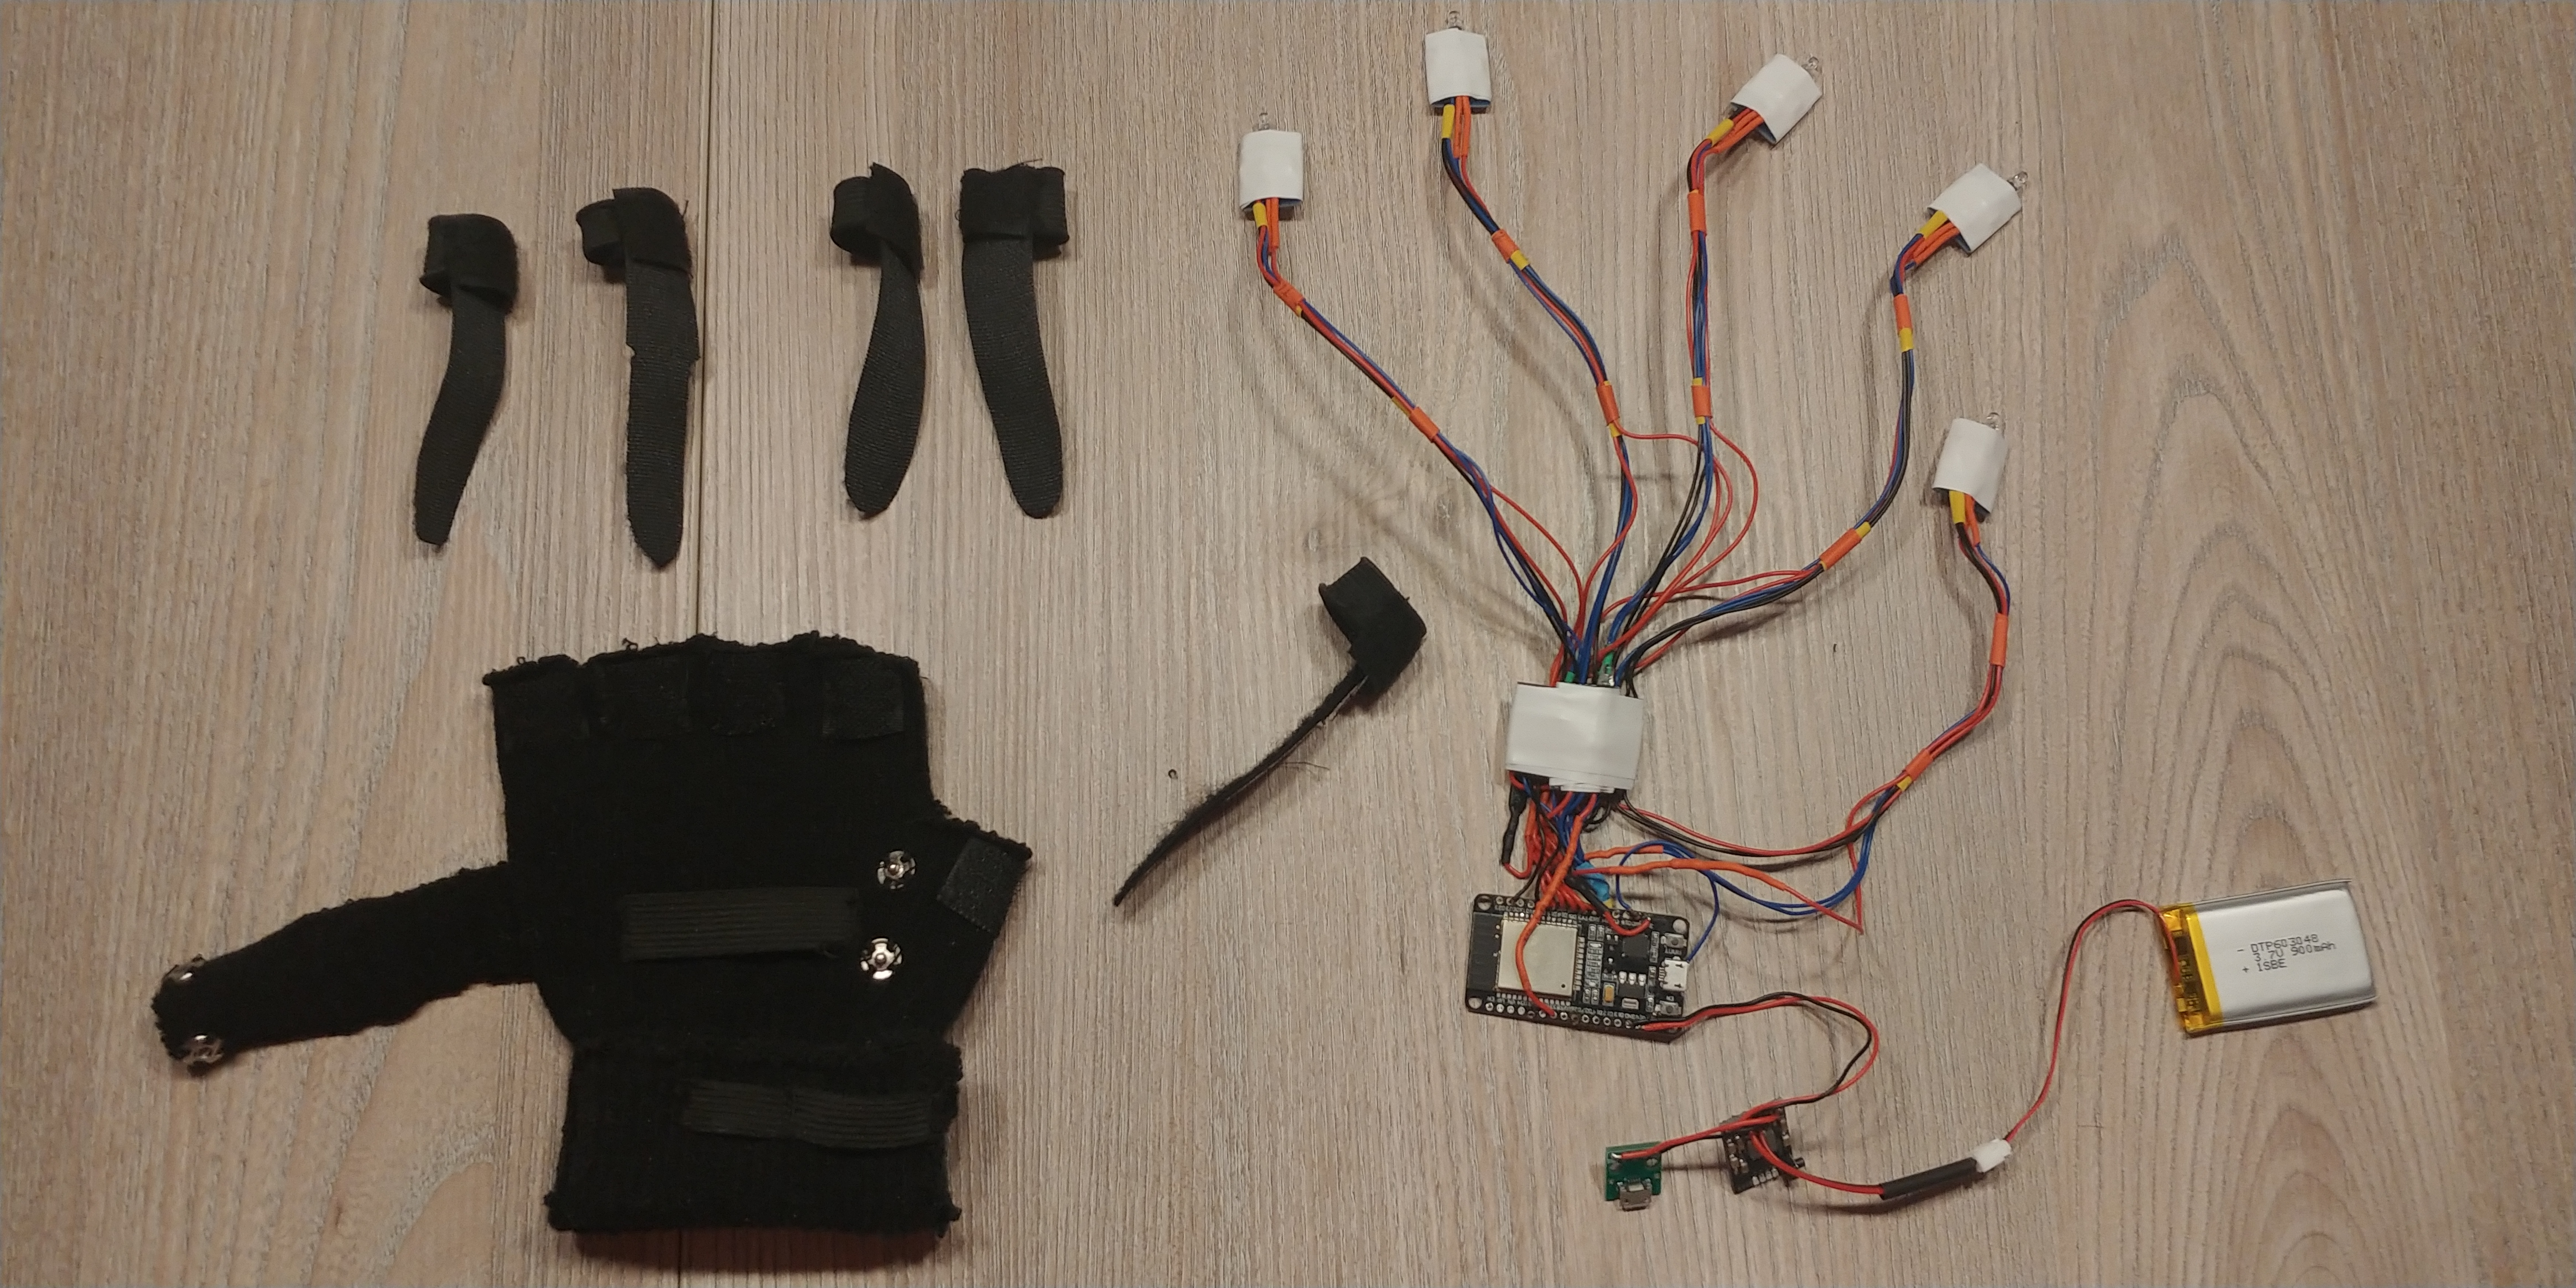
\includegraphics[width=1\columnwidth]{Bachelorarbeit/images/Exo.jpg}
    \caption{Handschuh neben dem Exoskelett und den lösbaren Fingerhalterungen}
    \label{fig:Exo}
\end{figure}

\begin{figure}[h]
	\centering
    \includegraphics[width=1\columnwidth]{Bachelorarbeit/images/FullView.jpg}
    \caption{Komplett Ansicht des Datenhandschuh}
    \label{fig:FullView}
\end{figure}

\chapter{Software}
Dieser Abschnitt wird auf die Implementation der Software eingegangen und es werden die wichtigsten Schritte behandelt, die für die Datenversendung und Verarbeitung entscheidend waren.
\section{Prozessor Setup}

Das Setup beider Prozessor Boards ist aus Vereinheitlichung identisch, bis auf das Abrufen der spezifischen IMUs wurden alle Programmierabschnitte gleich geschrieben. 
\\
Dabei wurden folgende Bibliotheken ausgesucht:
\begin{itemize}
    \item \textbf{Adafruit MPU6050} von Adafruit Industries, erlaubt das lesen von Daten aus dem MPU-6050\parencite{web:Adafruit}
    \item \textbf{DFRobot BMI160} von DFRobot Shanghai, erlaubt das lesen von Daten aus dem BMI160 \parencite{web:DFRobot}
    \item \textbf{MPU9250} aus der Arduino Bibliothek, erlaubt das lesen von Daten aus dem MPU-9250
    \item \textbf{UDPConnection} eine selbst entwickelte, ausschließlich für dieses Projekt implementierte Bibliothek, erlaubt UDP Pakete oder Daten Serial zu versenden 
\end{itemize}

Das \lstinline{Setup()} für die Initialisierung des ESP32 beginnt mit dem überprüfen der Verbindungsart, ob es sich um eine direkte Verbindung über den USB Port oder das Netzwerk handelt. Dieses entscheidet ob der Prozessor die Daten über den Serial Port oder die WiFi Verbindung, als UDP Paket versendet und erlaubt somit, unabhängig von Verbindung, Zugang auf die Daten zu gewähren. Das UDP Protokoll ist ein Kommunikationsprotokoll, welches eine Verbindung zwischen Anwendungen im Internet erstellt.
Durch das senden der Daten ohne jeglichen empfangenden Host ist dieser eine schnelle und zeitkritische Kommunikation, welche für kleinere Pakete die versendet werden sehr vorteilhaft sind, da diese ohne Zeitverzögerung das Ziel erreichen können. Die Pakete werden mit definierten Header versendet, den Ursprungs Port, den Ziel Port, die Paket Länge und einer Prüfsumme, wobei jedes Feld 2 Byte groß ist. 
\\
\\
In Kapitel \ref{MUX} wurde auf die limitierten Zugänge der $I^{2}C$ Ports eingegangen, dabei wurde der \textit{TCA9548A} als Erweiterung dieser hinzugefügt. Die Funktion \lstinline{tcaselect(uint8_t i)} erlaubt es uns somit die Ports direkt auf dem \textit{TCA9548A} aufzurufen, jedoch kann sich dieses als sehr ungeeignet wegen der statischen Struktur für die Architektur auswirken und für zukünftige Weiterentwicklung problematisch stellen.
Dafür wurde die Funktion \textit{identifyIMU()} hinzugefügt, welche alle Ports des MUX auf verfügbare Adressen prüft. Beim auffinden einer Verbindung, abhängig der Adresse wird der Port aufgerufen und entsprechend des verfügbaren IMU Modells initialisiert. Durch die zwei weitern Ports ist es möglich weiter Sensoren zu Datenerfassung anzuschließen, ohne die Limitierung des ESP32 in kauf zu nehmen.
\begin{lstlisting}
void identifyIMU(){
  for (uint8_t t=0; t<8; t++) {
      tcaselect(t);
      Serial.print("TCA Port #"); Serial.println(t);

      for (uint8_t addr = 0; addr<=127; addr++) {
        if (addr == TCAADDR) continue;

        Wire.beginTransmission(addr);
        if (!Wire.endTransmission()) {
          Serial.print("Found I2C 0x");  Serial.println(addr,HEX);
          if(addr != 0xC){
          initMPU(t);
}}}}}
\end{lstlisting}

Um die Kommunikation zwischen Host-PC und den beiden Handschuhen ohne Unterscheidung zu gewähren, versenden beide die gleiche Datenstruktur, das erlaubt uns eine identische Datenübertragung, ohne auf das Sensormodell zu achten. 
\\
\\
Die abgelesenen Daten werden kontinuierlich in der \lstinline{loop()} Anweisung ausgegeben, dabei wird sicher gegangen das jeder Port überprüft wird, falls noch weitere IMUs angebracht werden. Während des Initialisierungs Prozess werden die Ports, welche mit einem Sensor belegt waren innerhalb eines Arrays auf ein Wert gesetzt, hierfür steht eins für einen Finger oder drei für die Mittelhand. 
\begin{lstlisting}
void loop(){
  for(uint8_t i=0; i<8; i++){
        if(foundIMU[i] == 1 && readMPUFinger(i, buffer, seq)){
            udp.sendImuData(fingers ,buffer, i);
            seq = (seq + 1) % 255; 
        }else if(foundIMU[i] == 3 && readMPUCore(i, buffer, seq)){
            udp.sendImuData(palm, buffer, i);
            seq = (seq + 1) % 255; 
}}}
\end{lstlisting}
Mit der \lstinline{readMPU} Funktion werden die Daten innerhalb des Parameters \textit{buffer} gefüllt und über die UDPConnection Bibliothek auf dem Serial Port geschrieben oder mit einer UDP Datei verschickt.


\section{ROS System}
Um diese Daten in ablesbare Messungen zu wandeln, werden sie über das ROS System verarbeitet. ROS steht für Robotic Operating System, dieses besitzt verschiedene Bibliotheken und Funktionen mit denen es möglich ist Programme zu entwickeln die für die Robotik bestimmt sind. 
Sie können Daten übernehmen, die aus unterschiedlichen Sensoren gewonnen werden und konvertieren diese um in geordneten Daten, beispielsweise für die Orientierung, Analyse und Erfassung der Umgebung. 
\\
\\
\includegraphics[width=0.7\columnwidth]{Bachelorarbeit/images/Host-Architektur.drawio.png}
\\
\\
Um die versendeten Werte gebräuchlich zu formatieren, können diese zuerst in der folgenden Datenstruktur um konvertiert werden. 
\begin{lstlisting}[label=lst:structure]
IMU{
std_msgs/Header header
geometry_msgs/Quaternion orientation
float64[9] orientation_covariance
geometry_msgs/Vector3 angular_velocity
float64[9] angular_velocity_covariance
geometry_msgs/Vector3 linear_acceleration
float64[9] linear_acceleration_covariance
}
\end{lstlisting}
Diese Konvertierung wird in der \lstinline{convertPublisher} Klasse bewerkstelligt, hierbei werden alle Finger einem Topic zugeteilt. Ein Topic ist eine benannte Aufgabe, über die Nodes Nachrichten austauschen können. Diese Nodes besitzen Publisher oder Subscriber, die ihre Informationen an andere weitergeben oder empfangen können. Wird ein Node ausgeführt können die Topics über diverse Mittel abgelesen oder gespeichert werden.
\\
In den Folgenden Messungen wurden die Handschuh ohne Bewegung und ohne die Position festzulegen gemessen. 

\begin{figure}[h]
	\centering
    \includegraphics[width=1\columnwidth]{Bachelorarbeit/images/160-9250-RawData.png}
    \caption{Rohdaten des MPU-9250(links) und dem BMI160(rechts)}
    \label{fig:RawData160}
\end{figure}
Die Datenqualität des BMI160 Handschuh ist qualitativ Gut, es ist erkenntlich dass die Frequenz auf dem Handschuh gering ist. Durch Messungen der Datenrate wurde ermittelt das der BMI160 mit lediglich $8 Hz$ arbeitet, welches für das ermessen von Handbewegung nachteilig ist. 
\newpage
\begin{figure}[h]
	\centering
    \includegraphics[width=1\columnwidth]{Bachelorarbeit/images/6050-9250RawData.png}
    \caption{Rohdaten des MPU-9250(links) und dem MPU-6050(rechts)}
    \label{fig:RawData6050}
\end{figure}
Der MPU-6050 Handschuh besitzt durch seine stärkere Leistung eine höhere Frequenz von $80 Hz$, das 10-fache des BMI160. Die Gravitationswerte für den MPU-6050 werden auf die Beschleunigung noch eingewirkt, dass hat die Konsequenz der verschobenen Werte.

Alle drei IMUs versenden lediglich nur die Beschleunigung und die Winkelgeschwindigkeit, bis auf den MPU-9250, der auch die Kompassdaten misst. Eines der Ziele für den Datenhandschuh war es das aufzeichnen der menschlichen Handbewegung, dafür wird die Orientierungen der Sensoren benötigt um die relative Position zu bestimmen. Zur Lösung dieses Problems wurde der Madgwick Filter verwendet. Der Madgwick Filter \parencite{Madgwick} fusioniert die Winkelgeschwindigkeit mit der Beschleunigung, optional auch den Kompass, um aus diesen Werten die Orientierung zu errechnen.
\\
Der Madgwick Filter ist ein Filteralgorithmus, welcher von Sebastian Madgwick entwickelt wurde. Für die Bestimmung der Orientierung gibt es zwei Möglichkeiten. 
Die Bestimmung der Orientierung nur mit der Winkelgeschwindigkeit ist ausführbar, jedoch für die präzise Ermittelung wird die Ausgangsorientierung benötigt, da sonst lediglich eine relative Orientierung zum Raum errechnet wird. Mit Hilfe der Beschleunigung, bzws. dem Magnetfeld wird das Gravitationsfeld oder auch das Magnetfeld der Erde bestimmt. Über diesen Vorgang kann die absolute Orientierung gemessen werden.
\\
Um den Madgwick Filter einzusetzen verwendet ROS das \lstinline{imu_filter_madgwick} Paket. Die verschiedenen Parameter die das Paket verwendet, werden über die ROS APIs aufgerufen. Sie können verwendet werden um den Gravitationsvektor zu entfernen, das Verstärken des Filters \lstinline{gain} mit dem höhere Werte zu einer schnelleren Konvergenz bestimmt werden, jedoch auch größerem Rauschen. Um die Parameter für die Finger zu definieren, so dass diese auch einzeln Topics zugehören, wird alles über eine launch Datei ausgeführt.
\\
\begin{lstlisting}
<node pkg="imusensor" type="convertPublisher.py" 
    name="convertedIMUData"/>

<node pkg="imu_filter_madgwick" type="imu_filter_node" 
    name="dataglove_filter_imu_{imuID}" output="screen">
    <param name="world_frame" value="enu"/>
    <param name="fixed_frame" value="world"/>
    <param name="use_mag"     value="false" />
    <param name="publish_tf"  value="true" />
    <param name="reverse_tf"  value="false" />
    <param name="constant_dt" value="0.0" />
    <param name="orientation_stddev" value="0.8"/>
    <param name="remove_gravity_vector" value="true"/>
    <!-- Parameter for the BMI Glove
    <param name="gain" value="1.0" />
    <param name="gain" value="0.0" />
    -->
    <!-- Parameter for the MPU
    <param name="gain" value="1.0" />
    <param name="gain" value="0.0" />
    -->
    <param name="gain" value="0.3" />
    <param name="zeta" value="0.1" />
    <remap from="/imu/mag" to="/imu_event_{imuID}_converted_mag/imu/mag" />
    <remap from="imu/data_raw" to="/imu_event_{imuID}_converted/imu/data_raw"/>
    <remap from="imu/data" to="/imu_event_{imuID}_converted/imu/data_fused"/>
</node>
\end{lstlisting}
Zu Beginn muss der Publisher starten, dabei werden die Datenprotokolle über 
\\
den \lstinline{convertPublisher.py} empfangen, in die zugehörige Datenstruktur\ref{lst:structure} konvertiert und publiziert. Dann muss man die Parameter, die in der Launch Datei gesetzt wurden, auf den jeweiligen Sensor anpassen. \newpage
Für den MPU-6050 ist die lineare Beschleunigung noch ungenau, da die Erdanziehungskraft auf die Sensoren einwirkt.

\begin{figure}[h]
	\centering
    \includegraphics[width=1\columnwidth]{Bachelorarbeit/images/RemovalOfGravity.png}
    \caption{MPU-6050: Madgwick Filter ohne(oben) und mit(unten) Entfernung der Erdanziehungskraft}
    \label{fig:RemovalOfGravity}
\end{figure}
Mit dem Parameter \lstinline{remove_gravity_vector} ist der Filter in der Lage die Erdanziehungskraft aus der linearen Beschleunigung ungefähr auszurechnen und zu stabilisieren. 
\newpage
Nach Anwendung des Filters können somit auch die relativen Orientierungsdaten ermittelt werden.

\begin{figure}[h]
	\centering
    \includegraphics[width=1\columnwidth]{Bachelorarbeit/images/6050-Orientierung.png}
    \caption{Orientierungsdaten des MPU-9250(links) und MPU-6050(rechts)}
    \label{fig:Orientation6050}
\end{figure}
Dabei ist erkenntlich das die Kalibrierung noch nicht optimiert ist und nach einer Weile im Raum driftet, dafür werden jedoch rauschfreie Werte ausgerechnet. 

\newpage
\begin{figure}[h]
	\centering
    \includegraphics[width=1\columnwidth]{Bachelorarbeit/images/160Orientierung.png}
    \caption{Orientierungsdaten des MPU-9250(links) und MPU-6050(rechts)}
    \label{fig:Orientation160}
\end{figure}
Der BMI160 berrechnet durch die niedrige Datenrate sehr unruhige und auch driftende Werte im Raum. Dieses war durch die langsame Datenrate \ref{fig:RawData160} vorherzusehen, denn für die Ermittelung können schon langsame Schwingungsbewegung zu einer Fälschung der Orientierung führen, hier wurde der Sensor nicht bewegt und trotzdem sind die Daten mit viel Rauschen erkenntlich.

\newpage
Die MPU-9250 Orientierungsberechnung ohne und mit Verwendung des Magnetometerwertes zeigt deutliche Unterschiede der Orientierung.

\begin{figure}[h]
	\centering
    \includegraphics[width=1\columnwidth]{Bachelorarbeit/images/ComparisonMagValueSetTrueAndFalse.png}
    \caption{Vergleich der Orientierung beim einsetzen und ohne das einsetzen der Magnetometerwert}
    \label{fig:MagTrueAndFalse}
\end{figure}
Die Werte driften stärker ab, wenn die Magnetometerwerte nicht mit verwendet werden. Dieses zeigt eine gute Stabilität und genauere Orientierung mithilfe der Kompassdaten. 
\chapter{Bewertung}

\section{Handschuh Qualität}

Die Sensoren liegen fest auf den Fingern und werden auch bei schnellerer Bewegung nicht lose. Sie können auch durch ihre austauschbaren und anpassbare Fingerhalterungen auf die eigene Fingerlänge oder Größe angepasst werden und gibt somit größeren Spielraum für den Komfort. Durch das anbringen des MPU-9250 auf dem Multiplexer ist dieser sehr anfällig auf Fehler, da die Kabel verbunden mit den IMUs den Multiplexer mit bewegen, welches auch den MPU-9250 beeinflusst. 
Die drahtlose Verbindung wirkt sich positiv auf den Bewegungskomfort aus, denn somit wird dieser nicht durch die Länge des USB-Kabels eingeschränkt. 
Der Handschuhe besteht aus 100\% Baumwolle und wird somit auf längere Zeit warm, er liegt gut auf der Hand, jedoch wurde der Handschuh durch Einbindung der vielen Module sehr kompliziert und die Verkabelung wurde unübersichtlich. Durch die eingeschränkten Fläche auf dem Handschuh erwies sich die Platzierung der Module also als schwierig und kann den Nutzen Einschränken. 
Durch die feinen Kabel sollte der Handschuh auch mit Vorsicht gehandhabt werden, da die Kabel sehr fein und empfindlich sind. Für einen Prototypen, welcher die Charakteristiken der Handbewegung ermitteln soll reicht dieser aber aus.
\begin{figure}[h]
	\centering
    \includegraphics[width=1\columnwidth]{Bachelorarbeit/images/FullView.jpg}
    \caption{Komplett Ansicht des aktiven Datenhandschuh betrieben mit dem eingebauten Akku}
    \label{fig:FullView}
\end{figure}



\section{Datenqualität}
Die Datenqualität unterscheidet sich durch die verschiedene Datenrate stark, dabei hat der MPU-6050 eine Frequenz von $80 Hz$, also das 10-fache vom BMI160.
Wegen der eigentlichen Konstruktion des BMI160, welcher eigentlich für 
niedrigere Leistungskraft, aber genauere Werte spezialisiert. 
Die Rohdaten beider Handschuhe geben im Gesamten eine gute Performanz, wobei der BMI größeres Rauschen \ref{fig:RawData160} misst. 
Die Orientierung konnte mithilfe des Madgwick Filters errechnet werden, jedoch zeigt dieser Drift werte, für beide Datenhandschuhe. 
Der MPU-9259 hatte aber im Gegensatz zu den beiden anderen IMUs den Vorteil einen integrierten Kompass zu haben, durch die Anwendung des Filters in Abhängigkeit der Kompassdaten wurden die Drifts \ref{fig:MagTrueAndFalse} nicht mehr so stark wie ohne die Verwendung des Filters. Diesen somit als Haupt-IMU auf der Mittelhand zu setzen zeigte somit eine starke Stabilisierung der Daten und eine bessere Auswertung der Orientierung.
\chapter{Zusammenfassung}



Die heutige Technik besitzt mittlerweile viele technologische Errungenschaften um die charakteristische Bewegung verschiedener Körperteile zu ermitteln. Jedoch gehört die Hand mit ihren Fingern zu den Bereichen, die noch keinen richtigen Durchbruch erreicht haben, dabei bin ich auf einige der weiterentwickelten Modelle gestoßen, wie dem Manus Prime II und dem Forte Data Glove. \ref{alternativeDatenhandschuhe}
\\
Das Ziel dieser Bachelorarbeit war es zwei Datenhandschuhe zu gestalten und entwickeln, mit denen es möglich ist die charakteristische Bewegungen der Hand und den Fingern zu ermitteln. Dabei wurden der BMI160 und der MPU-6050 im Vergleich gestellt. Der Handschuh wurde auf Modularität entwickelt und mit den austauschbaren und auf die Länge anpassbaren Fingerhalterungen auf unterschiedliche Handtypen eingestellt.
\\
\\
Für die Qualität der beiden Fingersensoren sind einige Unterschiede aufgekommen.
Der BMI160 zeigte das dieser für den Gebrauch von solch einer hohen Auslastung nicht geeignet wäre, da sich die niedrige Datenrate auf die Qualität der Messungen bemerkbar macht und anschließend Orientierungswerte ausgibt mit starkem Rauschen.
Der MPU-6050 zeigte jedoch starke Punkte für den Gebrauch als Datenhandschuh, da dieser eine hohe Datenrate und mit vernünftigen Werten arbeitet. Die Anwendung des Madgwick Filters erlaubte uns die relative Orientierung zu errechnen, dabei stießen wir auf die Erkenntnis das dieser nach eine Weile stark driften kann, jedoch zeigte der MPU-9250, das die Kompassdaten der Orientierung dabei aushilft weniger zu driften und stärker zu stabilisieren.\ref{fig:MagTrueAndFalse}
\\
\\
Für zukünftige Weiterentwicklungen haben beide Handschuhe noch viele Verbesserungsmöglichkeiten. Für bessere Orientierung könnten die IMUs kalibriert werden oder die Messungen könnten mit einem kamerbasierten Ansatz und mithilfe der LEDs wirksamer getrackt werden. 
\cleardoublepage


\printbibliography[keyword=article]

\listoffigures
% ERKLÄRUNG
\input{Bachelorarbeit/_eidversicherung}
    
\end{document}